\documentclass[11pt]{article}
\usepackage[a4paper,width=150mm,top=25mm,bottom=25mm,bindingoffset=6mm]{geometry}
\usepackage{fancyhdr}
\pagestyle{fancy}
\usepackage[final]{graphicx}
\usepackage{subcaption}
%\usepackage{bera}% optional: just to have a nice mono-spaced font
\usepackage{listings}
\usepackage{xcolor}

\colorlet{punct}{red!60!black}
\definecolor{background}{HTML}{EEEEEE}
\definecolor{delim}{RGB}{20,105,176}
\colorlet{numb}{magenta!60!black}

\lstdefinelanguage{json}{
    basicstyle=\normalfont\ttfamily,
    numbers=left,
    numberstyle=\scriptsize,
    stepnumber=1,
    numbersep=8pt,
    showstringspaces=false,
    breaklines=true,
    frame=lines,
    backgroundcolor=\color{background},
    literate=
     *{0}{{{\color{numb}0}}}{1}
      {1}{{{\color{numb}1}}}{1}
      {2}{{{\color{numb}2}}}{1}
      {3}{{{\color{numb}3}}}{1}
      {4}{{{\color{numb}4}}}{1}
      {5}{{{\color{numb}5}}}{1}
      {6}{{{\color{numb}6}}}{1}
      {7}{{{\color{numb}7}}}{1}
      {8}{{{\color{numb}8}}}{1}
      {9}{{{\color{numb}9}}}{1}
      {:}{{{\color{punct}{:}}}}{1}
      {,}{{{\color{punct}{,}}}}{1}
      {\{}{{{\color{delim}{\{}}}}{1}
      {\}}{{{\color{delim}{\}}}}}{1}
      {[}{{{\color{delim}{[}}}}{1}
      {]}{{{\color{delim}{]}}}}{1},
}


%Gummi|065|=)
\title{\textbf{Virtual Parking System}}
\author{Luca Accorsi}
\date{}
\begin{document}

\maketitle

\section{Overview}
This application should be a working prototype of a system that aims to manage a smart parking area. The system is virtual in the sense that the components (sensors, cars, etc) are not real but are software components that simulate a plausible behavior.

\section{Requirements}
The XYZ industry requires the development of a parking system of approximately some hundreds of parking place. A park is a n x m matrix where each cell could be a parking place or a street block. The park designers will take care to design a drivable park, that is a park where drivers are able to move. Each parking place contains a parking sensor able to sense it in order to acquire information about the presence or absence of a car. The sensor is handled by a small computer equipped with a network interface that could be used to connect to networks. Each sensor has also the possibility to create very small local network useful to communicate with neighbors (other sensors or clients). The system should give drivers the possibility to quickly identify a free near parking place and to locate a previously parked car. It is thus required a client application that will be used by customers. To promote the distributed and decentralized vision of the industry it is also required that the parking system should be able to work in both a centralized way but it should also be able to perform some basic functionality in a fully distributed way.

\section{Requirements analysis}
From the requirements analysis can be state that the main entities that compose the system are:
\begin{itemize}
\item an \textbf{environment}: it is where the park area is placed and everything takes place. It is a grid-based place, that is an (n x m) matrix where each cell could be a street block or a parking place.
\item a \textbf{sensors layer}: each car parking place is equipped with a parking sensor able to determine if the place is free or busy, a computing processor and a network interface.
\item a \textbf{server application}: since the system should work in a centralized way, a central server (or many of them) is required.
\item some \textbf{client applications}: that an applications that a drivers will use to identify a free near parking place or to locate a previously parked car.
\end{itemize}
The main functions that the system has to accomplish could be summarized with:
\begin{itemize}
\item providing parking support
\item provide some basic information when the server is not available
\end{itemize}

The system should face the following complexity aspects:
\begin{itemize}
\item it is composed by a dynamic and possibly large set of components. At a given moment the number of clients is unpredictable.
\item it is open, that is components (clients but also sensors) could be added or removed while the system is working.
\item it is heterogeneous, clients, server and sensors application may be written in different programming languages.
\item it should work in a centralized and decentralized/distributed way.
\item the interactions are asynchronous and loose coupled.
\item the components are situated in a (virtual) world.
\end{itemize}

\section{Problem analysis}
The problem analysis could start from a very high level view. From the requirements could be stated that the whole system, from the \textbf{structure} point of view, is composed by the following sub-systems:
\begin{itemize}
\item the sensors spread across the park
\item the clients
\item a server
\end{itemize}
The whole system expected \textbf{behavior} is thoroughly explained in the requirements section but the behavior of each subsystem will be deeply analyzed in the following sub-sections. The \textbf{interactions} that occurs in the system may be initially introduced in a simplified version by the Figure 1. Here could be seen that exists two different kind of possible interactions: global (\textbf{g}) and local (\textbf{l}) ones. For global interaction it is meant an interaction that exploit a centralization element reachable independently from its physical distance, the server in this case, while a local interaction is an interaction that could happen in a well defined and typically small area, for eg. sensor-sensor or client-sensor communication.  

\begin{figure}
  \centering
	\includegraphics[scale=1]{system}
  \caption{High level system view}
\end{figure}

In the following subsections there will be a more focused analysis of each sub-system.
\subsection{Sensor model}
Each parking place is provided of a parking sensor, from now it will be called just sensor, able to perform the above described functionalities. The sensor is a simple proactive entity composed by two parts: the sensing unit and the control unit. The sensing unit is the software component that drives the physical (or virtual) input device (for eg. a proximity or obstacle physical sensor) while the control unit is the component where the application logic resides and that controls the sensing unit. The behavior of the sensor could discussed on two different levels. The server-oriented behavior could be described by an infinite loop where sense, process, act operations are performed. In particular the sense operation retrieve data from the sensing unit, the process operation adapt, change, translate the data in some kind of information (for eg. a json message) and the act operation uses some actuator to produce an effect (for eg. message sending using the network interface). An informal picture could be seen in Figure 2.

\begin{figure}
  \centering
	\includegraphics[scale=1]{sensor_server_oriented_behavior}
  \caption{Server-oriented sensor behavior}
\end{figure}
In the neighbor-oriented behavior, the sensor should be able receive requests from clients, check if it is able to satisfy them, if not spread the request to neighbor sensors. An informal picture could be seen in Figure 3.
\begin{figure}
  \centering
	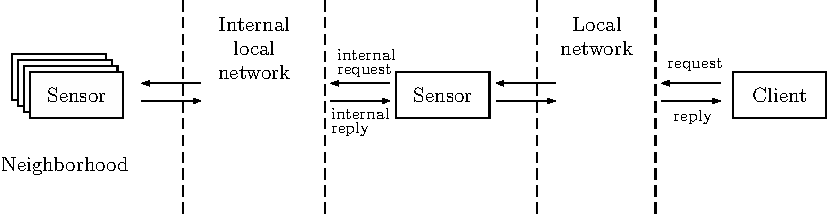
\includegraphics[scale=1]{sensor_neighbor_oriented_behavior}
  \caption{Neighbor-oriented sensor behavior}
\end{figure}
The two behaviors should of course be integrated and work together.

\subsection{Server model}
The server is a centralization element and a complex proactive and reactive entity, it receives state messages from the sensors and requests from clients. The server can build a complete view of the park, since it receives information from sensors, and update it when necessary. The server could be seen in a simplified way as composed by a sensors-handler module and a client-handler module. The sensors-handler module receives messages from sensors and update the internal server state while the clients-handler receives messages from clients. A client message is essentially a one-time welcome request where the client asks the server to send to it an updated version of the world. After the first request the client will never contact the server anymore. The server will publish new updated world versions each time the sensor-handler finds out that the server internal state has changed. An informal picture could be seen in Figure 4.
\begin{figure}
  \centering
	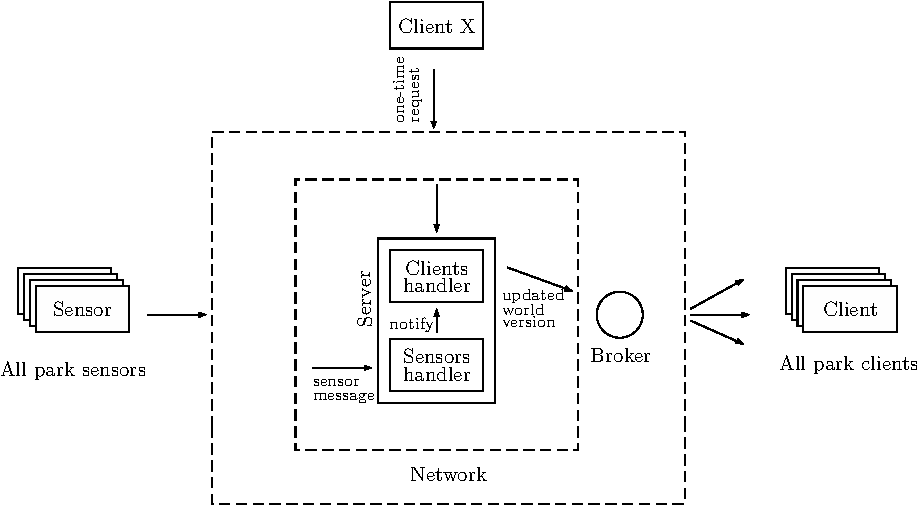
\includegraphics[scale=1]{server}
  \caption{Server behavior and interaction}
\end{figure}

\subsection{Client model}
Each driver is provided of an application that should grant him some smart parking support. The application should help to find out a near free place and to locate a previously parked car. The client application, from now on just client, is a \emph{thick} client composed by a user-interaction module, a server-interaction module and an (emergency) neighbor-interaction module. The user interaction-module should handle the user actions that is park a car, remove a parked car, locate a previously parked car and find the nearest free parking place. The server-interaction module should contact the server for the one-time welcome handshake and update the internal client storage each time the server publishes a new world version. Finally, the neighbor-interaction module should provide support in local interaction with near sensors when the server is not available. An informal picture could be seen in Figure 5.
\begin{figure}
  \centering
	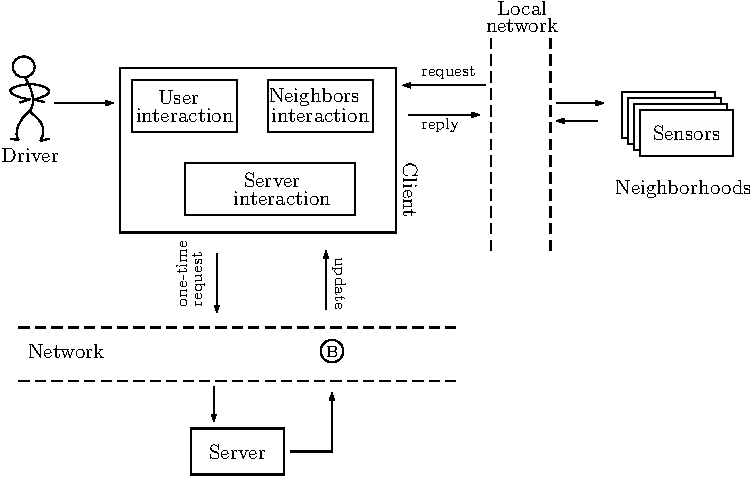
\includegraphics[scale=1]{client}
  \caption{Client behavior and interaction}
\end{figure}

\subsection{General remarks}

A parking sensor could be described as follows:
\begin{itemize}
\item structure: it is a composed entity, it contains a parking sensor and an application logic
\item interaction: the sensor periodically sends data to the server application, if the latter is available. The data is a JSON message defined as follows:

\begin{lstlisting}[language=json,firstnumber=1]
{
 "sensorId":"C1",
 "position": {
	"row":3,
	"column":5},
 "free":true
}
\end{lstlisting}

Fields description: \emph{sensorId} contains a unique sensor identifier, \emph{position} contains the place where the sensor is in the grid in terms of \emph{row} and \emph{column}, and \emph{free} is true if the parking place is not busy and false otherwise.

Each sensor sends a message like the one before also if the \emph{free} field isn't changed. This is the way the server knows that the sensor is correctly working.

The sensor could also handle the following local client requests:

\item behavior: the sensor sense the environment to check if the place is free or not and periodically sends this information to the server. It can also be contacted via local network, this time according to the client requests it checks if it is able to satisfy it (eg. it's free or it contains the client car) or forwards the request to neighbor sensors .
\end{itemize}

\subsection{Server model}

\subsection{Client model}

\subsection{Review of all possible interactions, message definitions and protocol definition}


\end{document}
